\documentclass{article} % article, report, book, slides, beamer, lettre, memoir
 
% =============================
% Import
\usepackage[francais]{babel}
\usepackage[T1]{fontenc}
\usepackage{fontspec} 
\newcommand\fr{\selectlanguage{francais}}
\usepackage{titlesec}
\usepackage{graphicx}
\usepackage{float}
\usepackage{amstext}
\usepackage{amssymb}
\usepackage{subcaption}
\usepackage{geometry}
\usepackage[colorlinks]{hyperref}
\usepackage{amsmath}
\usepackage{bbm}
\usepackage{blkarray}
\usepackage{empheq}

\newlength\dlf  % Define a new measure, dlf
\newcommand\alignedbox[2]{& {\settowidth\dlf{$\displaystyle #1$}\addtolength\dlf{\fboxsep+\fboxrule}\hspace{-\dlf}\boxed{#1 #2}}}
\geometry{
 a4paper,
 total={170mm,257mm},
 left=20mm,
 top=20mm,
 }


\newcommand\numberthis{\addtocounter{equation}{1}\tag{\theequation}}

\graphicspath{ {./static/} }

\newtheorem{theorem}{Theorem}
\newtheorem{mydef}{Definition}

\title{Mémoire Master 2: Probabilités et Statistiques  \\ Analyse spectrale des graphes et détection de structures de communauté dans les réseaux}
\author{Hugues-Vincent Ropert}
\date{Mai 2018}

\newcommand{\A}{\langle A \rangle}
% \newcommand{\example}{\textit{example} }

% \titleformat{\chapter}
%   {\Large\bfseries} % format
%   {}                % label
%   {0pt}             % sep
%   {\huge}           % before-code

\titleformat{\section}[block]
  {\fontsize{12}{15}\bfseries\sffamily}
  {\thesection}
  {1em}
  {}
\titleformat{\subsection}[block]
  {\Large\bfseries}
  {\thesubsection}
  {1em}
  {}


\begin{document}
\maketitle
\newpage

\tableofcontents
\newpage

\part{Introduction}
Lorem ipsum dolor sit amet, consectetur adipisicing elit, sed do eiusmod
tempor incididunt ut labore et dolore magna aliqua. Ut enim ad minim veniam,
quis nostrud exercitation ullamco laboris nisi ut aliquip ex ea commodo
consequat. Duis aute irure dolor in reprehenderit in voluptate velit esse
cillum dolore eu fugiat nulla pariatur. Excepteur sint occaecat cupidatat non
proident, sunt in culpa qui officia deserunt mollit anim id est laborum.
\part{Vue d'ensemble de la théorie du clustering spectral de graphes}
\section{La détection de communauté}
\subsection{Motivations}
La théorie des réseaux, a pour but d'analyser les graphes correspondant à des réseaux tels que celui de l'Internet, de la politique ou de la classification en biologie.
Chacun de ces graphes ont des propriétés spécifiques telles que:
\begin{itemize}
 	\item[-] \underline{Centrality}: mesure de cohésion du graphe ;
 	\item[-] \underline{``small world effect''}:  distance moyenne entre deux nœuds est proportionnelle au log du nombre de nœuds dans le graphe;
 	\item[-] \underline{Clustering}: mesure du regroupement des nœuds du graphe;
 	\item[-] \underline{Efficiency}: mesure la résistance du graphe;
 	\item[-] \underline{Degree distribution}; 
 	\item[-] \underline{Community Structure}.\\
 \end{itemize}
C'est cette dernière propriété qui va nous intéresser, à savoir la structure de communauté d'un graphe.
L'idée de communauté correspond à l'intuition selon laquelle il y a des nœuds qui ont un lien étroit et forment des sous ensembles de nœuds de ce graphe.
Par exemple dans le graphe des représentants politique Français, les hommes politiques d'un même partie appartiendraient à une même communauté.
Cependant, dans cet exemple les choses peuvent être plus subtiles que ça, c'est là qu'intervient la détection de communauté.

\subsection{Méthodes}
Il y a différentes classes de méthodes pour la détection de communauté, en voici une liste non exhaustive.
Pour une liste fournies des méthodes existante voir \cite{Community_detection_in_graphs}.
\begin{itemize}
	\item[-] Hierarchical clustering
	\item[-] Graph partitioning
	\item[-] Partitional clustering
	\item[-] Spectral clustering \\
\end{itemize}

\subsection{Comparaison des structures de communauté}
La notion de structure de communauté dans un graphe n'a pas de définition claire et consensuelle.
En effet, lorsque l'on veut faire de la détection de communauté nous cherchons d'hypothétiques lien entre les nœuds d'un réseau.
Cependant, ce lien ne peut pas avoir de sens a priori. 
Dans l'exemple du graphe du personnel politique français, si on trouve une certaine structure de communauté, quel sens peut-on donner au fait que deux personnes appartiennent à la même communauté.
Pour trouver un sens aux liens extraits par les algorithmes, on peut essayer de partir du sens de l'information à partir de laquelle le graphe a été construit, mais cela reste de l'ordre de l’interprétation.  

De plus, le résultat obtenu dépend entièrement du choix de la méthode utilisée.
La non unicité des résultats des algorithmes de détection de communauté rajoute une variabilité substantielle à l’interprétation d'une structure de communauté.
En substance, cela veut dire qu'en plus de choisir comment construire le graphe (i.e à partir de quelle information), il faut aussi choisir une métrique qui mesure la notion de proximité entre deux éléments du réseau.\\

Une conséquence négative de la non unicité des résultats est le fait qu'il n'existe pas de référence à partir de laquelle comparer les différentes structures de communautés obtenues.
Le seul moyen de juger le véracité des résultats obtenus est de les comparer entre eux et de faire une synthèse.
Il existe une abondante littérature sur la comparaison des méthodes.

On peut cependant essayer de comparer théoriquement les méthodes utilisés en analysant des graphes que l'on génère de manière aléatoire et dont on connaît les communautés.
On appelle ces graphes, ``graphe aléatoire'' ou `random graph'
Cette manière de procéder à l'avantage de posséder une référence à partir de laquelle comparer les algorithmes.
En revanche, les graphes générés ainsi ne correspondent pas forcement au graphes que l'on trouve dans la ``nature''.
Par conséquent des algorithmes qui ont de très bonnes performances sur un certain type de graphe, ne seront pas forcement pertinents sur des graphes générées à partir de données réelles. 

Une grande part de la recherche dans ce domaine est de rajouter des propriétés et des contraintes aux algorithmes de génération de graphes afin qu'ils satisfassent au mieux les propriétés des graphes que l'on observe dans la réalité (réseaux sociaux ...).
On peut donc ainsi trouver le meilleur algorithme pour un ensemble de graphes satisfaisant un certain nombre de propriétés.\\

Pour comparer les résultat a partir d'un graphe aléatoire il faut choisir une métrique.
Il existe une très grand nombre de métrique qui donnent là aussi des résultats divergeant.
On ne sait pas jusqu'à présent quel algorithme est le plus fiable.

Dans le cas où l'on utilise un graphe aléatoire, il existe plusieurs moyens de comparer les partitions obtenues avec la partition de référence.  
Pour une liste fournies des méthodes existante voir \cite[p.77-79]{Community_detection_in_graphs}.
Ci-dessous une liste non exhaustive des métriques qui seront utilisées ultérieurement.
\begin{itemize}
	\item[-] Fraction of correctly classified vertices ; 
	\item[-] Fowlkes and Mallows metric; 
	\item[-] Rand Index; 
	\item[-] Normalized Mutal Information; 
\end{itemize}

\subsection{Comparaison des performances}
Une autre problématique des algorithmes de détection de communautés est la performance.
En effet, beaucoup de méthodes considérées comme les plus efficaces du point de vue des communautés obtenues ont une complexité polynomiale voire exponentielle.
Or beaucoup de réseaux de vrai-monde ont un nombre de nœuds d'un ordre largement supérieur au milliard. 
On se retrouve donc dans le trade-off classique entre la performance et l'erreur d'approximation. 
Dans ces situations, il faut dont trouver des algorithmes à la fois performants et consistants.\\

C'est dans cette perspective que se place les papiers que nous étudions dans ce mémoire.
Nous nous placerons toujours dans le contexte d'un Stochastic Block Model, ou SBM, à 2 communautés de même taille et à deux probabilités $p_{in}$ et $p_{out}$.

Un SBM est un graphe aléatoire dans lequel on choisi un nombre de nœuds $n$, le nombre de communautés $q$. 
On génère ainsi une graphe à n nœuds sans arrêtes, et ensuite pour chaque pair de nœuds on simule une variable de Bernoulli pour décider si l’arrête existe ou non.
Le paramètre de la loi de Bernoulli est $p_{in}$ si les deux nœuds appartiennent à la même communauté et $p_{out}$ sinon.

Dans ce contexte, d'après le paragraphe \cite[Numerical results]{Spectral_Detection_in_the_Censored_Block_Model}, l'algorithme ``belief propagation'' est réputé pour être optimal sur les partitions rendues.
Ainsi, pour comparer les performances des algorithmes dans ce contexte, la littérature utilise cet algorithme comme un benchmark du point de vue de la répartition obtenue.
Ensuite ils comparent la performance et le temps d’exécution par rapport à celui-ci.
Ci-dessous une figure provenant de \cite{Spectral_redemption_clustering_sparse_networks} qui synthétise ce paragraphe.
\begin{figure}[H]
\centering
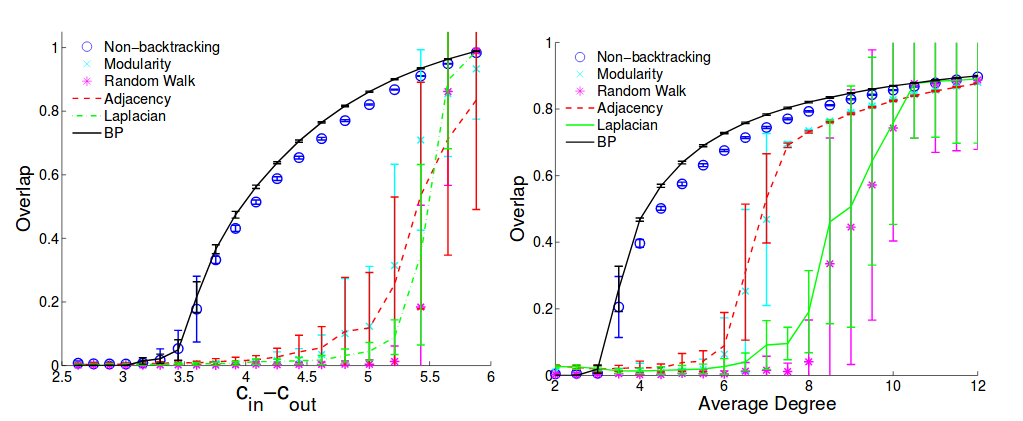
\includegraphics[scale=0.5]{static/bp_perf.png}
\caption{Précision des algorithmes de détection spectral basées sur différents opérateurs linéaires par rapport l'algorithme ``belief propagation''}
\end{figure}

\subsection{Perspectives}
Les limites des modèles spectraux qui sont en développement pour la détection de communauté sont les suivantes:
\begin{itemize}
	\item[1-] Seuil à partir duquel la méthode spectrale n'est plus en mesure de détecter le communauté ;  
	\item[2-] Temps de calcul sur de grands graphes;  
	\item[3-] Raffinement des modèles de communautés.  
\end{itemize}
\section{Spectral clustering}
L'idée centrale des techniques de clustering spectral est qu'un graphe est représentable par une matrice à partir de laquelle on peut utiliser les techniques d'analyse de l'algèbre linéaire.

Un graphe $G$ est la donnée d'un couple $(V, E)$ tel que $V$ est une ensemble de nœuds et $E$ et un ensemble d'arêtes (i.e un couple $(i,j)$ où $i,j \in V$).
A partir de cette définition on peut représenter le graphe par une matrice dont les éléments correspondent à certaines données de $G$.
Il existe tout un ensemble de matrices représentant le graphe:
\begin{itemize}
  	\item[-]  Adjencency Matrix $= A$;
  	\item[-]  Laplacian Matrix $= L$;
  	\item[-]  Modularity Matrix $= M$;
  	\item[-]  Bethe Hessian Matrix $= H$;
  	\item[-]  "$\alpha$-normalized” Adjacency Matrix $= D$.\\
\end{itemize}
Par exemple, la matrice d'adjacence d'un graphe, notée $A$, est définie telle que $\forall i,j \in V, \; A_{ij} = \mathbbm{1}_{(i,j) \in E}$.
Une colonne $i$ représente le nœud $i$ dont chaque composante, $j$, est égale à $1$ si il existe une arête entre $i$ et $j$ et $0$ sinon.\\

Ci-dessous un graphe qui permettant d'avoir une vue d'ensemble sur l'avancement des méthodes de spectrales de détection de communautés.
Cette liste n'est pas exhaustive.
\begin{figure}[H]
\centering
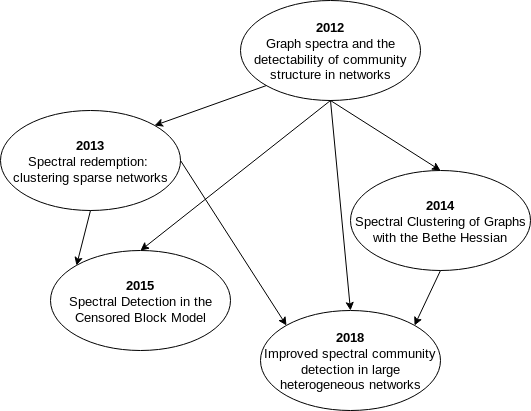
\includegraphics[scale=0.5]{static/graph_research.png}
\caption{graphe des différentes méthodes de ``graph spectral clustering''}
\end{figure}

\subsection{Algorithme de clustering spectral de graphe}
 \label{par:algo spectral clustering}
La procédure pour associer une communauté aux nœuds de $G$ via une méthode spectrale est la suivante: 
\begin{itemize}
	\item[1-] Calcul des vecteurs propres, $v_i$, d'une matrice représentant le Graphe $G$ ;
	\item[2-] Sélection des $l$ vecteurs propres portant l'information de la structure de communauté ; 
	\item[3-] Construction de la matrice $W = [v_1, \cdots, v_l] \in \mathbb{R}^{n\times l}$ ; 
	\item[4-] Projection des vecteur lignes $r_j$ de $W$ sur l'espace de dimension $l$, où chaque $r_j$ correspond  au nœud $j$ ; 
	\item[5-] Catégorisation des vecteurs $r_j $ dans une communauté via des algorithmes de clustering: \textit{K-Means}, \textit{Expetation-Maximization}, \textit{Support vector machine }, etc.\\
\end{itemize}

\par{\underline{Étape 1:}}
La matrice $A$ est carrée, par conséquent elle peut être interprétée comme la représentation d'un endomorphisme dans un espace X de dimension $n$ (nombre de nœuds dans $G$).
Soit la base canonique $(e_i)_{i=1:n}$, chaque $e_i$ correspond au nœud $i$.
Les vecteurs propres de $A$ sont donc des combinaisons linéaires des nœuds de $G$.
Les nœuds concernés ont donc une certaine dépendance.
\par{\underline{Étape 2:}}
Les entrées de la Matrice $A$ sont modélisées par des variables aléatoires vérifiant certaines hypothèses (e.g centrées, moments finis, indépendantes ...).
La théorie des matrices aléatoires nous dit qu’asymptotiquement la mesure spectrale de A converge vers une loi déterministe $\mu$ (loi qui dépend de la matrice étudiée).
Les valeurs propres de $A$ distribuées selon $\mu$ peuvent être interprétées comme du bruit lié aux fluctuations aléatoires des simulations.
Elles nous renseigne en rien sur la structure non aléatoire des entrées de $A$ .\\
Cependant, lorsque le graphe admet une structure de communauté, les entrées ne sont plus tout à fait indépendantes.
Dans ce cas de figure, la théorie prévoit que des valeurs propres sortent du support de la mesure spectrale $\mu$.
Ce sont ces valeurs propres qui contiennent l'information de la structure de communauté de $G$.\\
Autrement dit, si la structure de communauté de $G$ n'est pas assez ``explicite'', les valeurs propres censées porter l'information des communautés ne sortiront pas du support de la mesure spectrale théorique, et donc, seront interprétées comme du simple bruit.
Dans cette situation, la méthode spectrale est incapable de déceler la structure de communauté de $G$.
\par{\underline{Étape 4:}}
Les vecteurs colonnes de W correspondent à des combinaisons linéaires de nœuds.
De par la construction de A, les entrées $i$ de ces vecteurs colonnes sont la somme des arêtes entre les nœuds sous-jacent et le nœud $i$.
Les vecteurs propres que l'on a gardés sont ceux qui portent l'information des communautés.
Donc chaque vecteur ligne représente un nœud du graphe et l'espace dans lequel il se meut constitue l'information de la structure de communauté.\\

Les algorithmes de détection de communauté spectraux à partir des opérateurs linéaires tels que la matrice ``non-backtracking'' et la matrice ``Bethe Hessian'' sont similaires et sont décrits dans l'article \cite[Spectral detection in the censored block model]{Spectral_Detection_in_the_Censored_Block_Model}.


\part{Article: Graph spectra and the detectability of community structure in networks - Raj Rao Nadakuditi and M. E. J. Newman}
% \part{partie}
% \chapter{chapitre}
% \section{section}
% \subsection{sous-section}
% \subsubsection{sous-sous-section}
% \paragraph{paragraphe}
% \subparagraph{sous-paragraphe}
\section{Théorie}
\subsection{Contexte: Stochastic Block Model à 2 communautés}
Le but de ce papier est d'expliquer en détail la méthode de détection de communauté via la théorie spectrale de l'article de RR. Nadakuditi et M. E. J. Newmann.
C'est un article qui décrit les limites d'un modèle spectral dans un cadre spécifique à deux communautés.

Nous allons nous placer dans le contexte d'un Stochastic Block Model (SBM) à deux communautés (i.e \textbf{q}=2).
C'est un graphe \textbf{G} non orienté à \textbf{n} nœuds dont chaque arête entre deux nœuds suit une loi de Bernoulli de paramètre $p_{in}$ si les nœuds appartiennent à la même communauté et $p_{out}$ si les nœuds ne sont pas dans la même communauté.  

Nous noterons \textbf{A} la matrice d'adjacence du graphe \textbf{G}.
Elle est symétrique de par le fait que le graphe soit non orienté.
Nous supposerons d'ailleurs, que ses éléments sont rangés dans l'ordre de leur communauté.
Dans notre cas avec \textbf{q}=2, les $\mathbf{n}/2$ premières lignes correspondent aux noeuds de la communauté 1, et les $\mathbf{n}/2$ dernières la communauté 2.
Même chose pour les colonnes, par symétrie de \textbf{A}.\\
Cette disposition des éléments ne change pas le résultat final de l'analayse.
En effet, on sait que toutes les matrices congruentes représentes la même forme bilinéaire dans des bases différentes. 
Or le but de la procédure qui va suivre va être d'analyser la distribution des valeurs propres de notre matrice.
Par conséquent ranger les colonnes d'une matrice selon un ordre arbitraire correspond à la même forme bilinéaire et donc aux mêmes valeurs propres.\\

Chaque élément de la matrice \textbf{A} est simulé par une loi de Bernoulli avec: 
\begin{equation}\label{rq:probability}
 A_{ij} \sim \left\{
  \begin{array}{lr}
    B(p_{in}) & : (i,j < \frac{n}{2}) \; ou \; (i,j \ge \frac{n}{2}) \\
    B(p_{out}) & : else \; where
  \end{array}
\right.\nonumber
\end{equation}
\begin{equation} 
A_{ij} = A_{ji}\nonumber
\end{equation}


\subsection{Analyse spectrale de la matrice d'adjacence \textbf{A}}\label{ch:Analyse spectrale de la matrice d'adjacence}
L'idée générale de l'analyse spectrale qui va suivre est de nous ramener à un régime spectral de grande matrices aléatoires connu. 
Dans notre cas, nous verrons que le régime associé à notre matrice d'adjacence (SBM $\textbf{q}=2$) est celui du théorème de \textit{Wigner} avec perturbation de rang fini.
La trame sera la suivante:
\begin{itemize}
 	\item[1-] réécriture de la matrice $A = \langle A \rangle + X$;
 	\item[2-] étude de la mesure spectrale de X;
 	\item[3-] étude de la mesure spectrale de B où $B = X + P_1$;
 	\item[4-] étude de la mesure spectrale de $A = B + P_2 = X + P_1 + P_2$.
 \end{itemize} 
où $P_1$, $P_2$ sont des perturbations de rang 1 et $\langle A \rangle$ correspond à la moyenne de A du SBM.\\
% ------------------------------------------------- equation (1) -------------------------------------------------
\subsubsection*{1- Équation de $\langle A \rangle$}
En partant de $A$, on définit $\langle A \rangle$ comme la matrice dont les entrées $\langle A \rangle _{ij} = \mathbb{E}(A_{ij})$
Soit
\begin{align*}
	\langle A \rangle 
	&=
	\begin{bmatrix}
		p_{in} & p_{out}\\
		p_{out} & p_{in}\\
	\end{bmatrix} \otimes \mathbf{1}_{\frac{n}{2}}\mathbf{1}_{\frac{n}{2}}^T \times \frac{n}{2}\\
	&=
	\begin{bmatrix}
		c_{in} & c_{out}\\
		c_{out} & c_{in}\\
	\end{bmatrix} \otimes \mathbf{1}_{\frac{n}{2}}\mathbf{1}_{\frac{n}{2}}^T \times \frac{1}{2}\\
	&=\left(\frac{1}{2} \times
	\begin{bmatrix}
		c_{in} + c_{out} & c_{in} + c_{out}\\
		c_{in} + c_{out} & c_{in} + c_{out}\\
	\end{bmatrix} 
	+ \frac{1}{2} \times
	\begin{bmatrix}
		c_{in} - c_{out} & -c_{in} + c_{out}\\
		-c_{in} + c_{out} & c_{in} - c_{out}\\
	\end{bmatrix}
	\right) \otimes \mathbf{1}_{\frac{n}{2}}\mathbf{1}_{\frac{n}{2}}^T \times \frac{1}{2}\\
	&=\left(\frac{1}{2} (c_{in} + c_{out})\times \mathbf{1}_2\mathbf{1}_2^T
	+ \frac{1}{2} (c_{in} - c_{out}) \times \mathbf{u}_2\mathbf{u}_2^T
	\right) \otimes \mathbf{1}_{\frac{n}{2}}\mathbf{1}_{\frac{n}{2}}^T\\
	&= \frac{1}{2}(c_{in} + c_{out})\mathbf{1}_n\mathbf{1}_n^T + \frac{1}{2}(c_{in} - c_{out})\mathbf{u}_n\mathbf{u}_n^T \numberthis \label{eq:1}
\end{align*}
Avec
\begin{align*}
c_{in} &= np_{int} \\
c_{out} &= np_{out}\\
\mathbf{1}_n &= (\underbrace{1,\ldots,1}_{n\text{-times}})/\sqrt{n}\\
\mathbf{u}_n &= (\underbrace{1,\ldots,1}_{\frac{n}{2}\text{-times}}, \underbrace{-1,\ldots,1}_{\frac{n}{2}\text{-times}})/\sqrt{n}\\
\langle\mathbf{1_n}|\mathbf{u_n}\rangle &= 0
\end{align*}


À présent \textbf{A} peut être écrite sous la forme $A = \langle A \rangle + X$.
La matrice X est interprétable comme la déviation entre la matrice d'adjacence du graphe et sa moyenne.
La matrice X est par définition une matrice aléatoire symétrique à entrées indépendantes et de moyenne 0.
Essayons d'analyser sa mesure spectrale.
On a 

\begin{equation}
X = A - \langle A \rangle\nonumber
\end{equation}
\begin{equation}
	X_{ij}  = \left\{
	\begin{array}{lr}
		B_{ij}(p_{in}) - p_{in} & : (i,j < \frac{n}{2}) \; ou \; (i,j \ge \frac{n}{2}) \\
		B_{ij}(p_{out}) - p_{out} & : else \; where
	\end{array}
\right.\nonumber
\end{equation}
Où $B_{ij}(p) \sim B(p)$, $B(p)$ loi de Bernoulli de paramètre p et $B_{ij} = B_{ji}$\\


% ------------------------------------------------- 2- trouver X  -------------------------------------------------
\subsubsection*{2- Profil de variance de $\frac{X}{\sqrt{n}}$}
Nous aimerions modifier la forme des entrées $X_{ij}$ en $\sigma_{ij} Z_{ij}$, où $Z_{ij}$ est une variable aléatoire centrée réduite, afin de nous ramener à des théorèmes connus.

Pour $(i,j < \frac{n}{2}) \; ou \; (i,j \ge \frac{n}{2}) $ on a:
\begin{align*}
\mathbb{E}(X_{ij}) &= \mathbb{E}(B(p_{in}))- p_{in} = 0\\
\sigma_{in}^2 &= \mathbb{V}(X_{ij}) \\ 
			  &= \mathbb{V}(B(p_{in})) \\
			  &= p_{in} (1 - p_{in})
\end{align*}
même raisonnement avec $p_{out}$ 
\begin{align*}
\sigma_{out}^2 =  p_{out} (1 - p_{out})
\end{align*}
finalement on obtient 
\begin{equation}
	X_{ij} \sim \left\{
	\begin{array}{lr}
		\sigma_{in} Z_{ij} & : (i,j < \frac{n}{2}) \; ou \; (i,j \ge \frac{n}{2}) \\
		\sigma_{out} Z_{ij} & : else \; where
	\end{array}
\right.\nonumber
\end{equation}
Où $Z_{ij} = \frac{B(p) - p}{\sqrt{p(1-p)}} \;\;avec \; p = p_{in} \; ou \; p_{out}$\\

% ------------------------------------------------- théorème 1 -------------------------------------------------
Le théorème de Wigner ne fonctionne que pour les matrices à entrées iid. 
Il existe un théorème lorsque le profil de variance de la matrice aléatoire étudié est stochastique.
\begin{theorem}\label{th:1}
Soit $W \in M_{n}(\mathbb{R})$, $W_{ij}$ sont des variables aléatoires réels\\
On suppose que les $(W_{ij})_{i \leq j}$ sont indépendantes telles que $\mathbb{E}(W_{ij}) = 0$, $\sigma_{ij}^2 = \mathbb{E}(W_{ij}^2) < \infty$, $W_{ij} = W_{ji}$\\
On appelle profil de variance la matrice symétrique
\begin{align*}
	\tilde V_n = (\sigma_{ij}^2)_{1 \leq i,j \leq n}
\end{align*}
et profil de variance normalisé 
\begin{align*}
	V_n = \left(\frac{\sigma_{ij}^2}{n}\right)_{1 \leq i,j \leq n}
\end{align*}
On suppose que $V_n$ est stochastique: $\forall i = 1:n , \; \sum_{j=1}^{n}V_{ij} = \sigma^2$\\
Alors la mesure spectrale $L_{n}$ de $\frac{W}{\sqrt{n}}$ vérifie

\begin{equation}
	L_n\xrightarrow[n \to +\infty]{etr} \mathbb{P}_{wig}\nonumber \; p.s
\end{equation}\\
où $\mathbb{P}_{wig}$ est la loi de Wigner de densité $f_{wig}(x)= \frac{\sqrt{(4\sigma^2 - x^2)_+}}{2\pi\sigma^2}$
\end{theorem}

Soit $V$ le profil de variance de $\frac{X}{\sqrt{n}}$. $\forall i = 1:n$ on a: 
\begin{align*} 
\sigma_{i \cdot}^2 &= \sum_{j=1}^{n}V_{ij}  \\
 		&= \boxed{\frac{\sigma_{in}^2 + \sigma_{out}^2}{2} = \sigma^2}
\end{align*}
Si on note $\rho(x)$ la densité spectrale de $\frac{X}{\sqrt{n}}$ on a;
\begin{equation}
	\rho(x) = \frac{\sqrt{(2(\sigma_{in}^2 + \sigma_{out}^2) - x^2)_+}}{\pi(\sigma_{in}^2 + \sigma_{out}^2)}
\end{equation}

% ------------------------------------------------- 3- étude de B  -------------------------------------------------
\subsubsection*{3- étude de la mesure spectrale de $B$}
Dans la suite de l'étude nous noterons B la matrice de modularité telle que 
\begin{align*} 
B :&= X + \frac{1}{2}(c_{in} - c_{out})\mathbf{uu}^T \\
\frac{B}{\sqrt{n}} &= \frac{X}{\sqrt{n}} + \frac{1}{2\sqrt{n}}(c_{in} - c_{out})\mathbf{uu}^T\\
\end{align*}
Soit v le vecteur propre de $\frac{B}{\sqrt{n}}$ associé à $\lambda_{max}$ et soit $\Gamma = \frac{X}{\sqrt{n}}$

\begin{align} 
\frac{B}{\sqrt{n}}\mathbf{v} &= \lambda_{max}\mathbf{v} \nonumber\\
(\Gamma - \lambda_{max}I)\mathbf{v} &= -\frac{1}{2\sqrt{n}}(c_{in} - c_{out})\mathbf{uu}^T \mathbf{v} \nonumber\\
 \mathbf{u^Tv} &= -\frac{1}{2\sqrt{n}}(c_{in} - c_{out})\mathbf{u^T}(\Gamma - \lambda_{max}I)^{-1}\mathbf{uu}^T \mathbf{v} \nonumber\\
 1 &= -\frac{1}{2\sqrt{n}}(c_{in} - c_{out})\mathbf{u^T}(\Gamma - \lambda_{max}I)^{-1}\mathbf{u} \label{eq:3}
\end{align}

% ------------------------------------------------- Théorème de Wigner isotrope -------------------------------------------------
\begin{theorem}[Théorème de Wigner isotrope]\label{th:2}

Soit $W \in M_{n}(\mathbb{R})$, telle que $W_{ij}$ sont des variables aléatoires réels, $\mathbb{E}(W_{ij}) = 0$, $\mathbb{E}(W_{ij}^2) < \infty$, $W_{ij} = W_{ji}$, W à un profil de variance V tel que $\forall i = 1:n , \; \sum_{j=1}^{n}V_{ij} = \sigma^2$ pour $\sigma \in \mathbb{R}$\\
Soit $Q(z)$ la résolvante de W
\begin{align*} 
Q(z) = (W - zI)^{-1}\\
\end{align*}
Soient $\mathbf{u}$, $\mathbf{v}$ des vecteurs déterministes tels que $\|\mathbf{u}\|, \|\mathbf{v}\| < \infty$.\\
Alors 
\begin{align*} 
\mathbf{u}^*Q(z)\mathbf{v} - \langle \mathbf{u}, \mathbf{v} \rangle g_{wig}^{\sigma^2}(z) \xrightarrow[n \to +\infty]{} 0\\
\end{align*}
où $g_{wig}^{\sigma^2}$ est la transformé de Stieltjes de la loi de Wigner de paramètre $\sigma^2$ qui satisfait l'équation
\begin{equation}
	\sigma^2g_{wig}^{\sigma^2}(z)^2+\lambda_{max}g_{wig}^{\sigma^2}(z)+1=0
\end{equation}
\end{theorem}
Reprenons l’équation \eqref{eq:3}, en appliquant le Théorème de Wigner isotrope et en s'assurant que tous les termes de droite convergent, nous avons:
\begin{align*}
\mathbf{u^T}(\Gamma - \lambda_{max}I)^{-1}\mathbf{u} \xrightarrow[n \to +\infty]{} g_{wig}^{\sigma^2}(\lambda_{max})
\end{align*}
or $g_{wig}^{\sigma^2}(\lambda_{max})$ satisfait l'équation suivante 
\begin{align}
	\sigma^2U^2+\lambda_{max}U+1=0 \implies U = \frac{- \lambda_{max} \pm \sqrt{(\lambda_{max}^2 - 4\sigma^2)}}{2\sigma^2}
\end{align}
Donc
\begin{align}
	\eqref{eq:3} &\Leftrightarrow1 = -\frac{1}{2\sqrt{n}}(c_{in} - c_{out}) g_{wig}^{\sigma^2}(\lambda_{max}) \nonumber\\
	&\Leftrightarrow 1 = -\frac{1}{2\sqrt{n}}(c_{in} - c_{out}) \frac{- \lambda_{max} - \sqrt{(\lambda_{max}^2 - 4\sigma^2)}}{2\sigma^2} \nonumber\\
	&\Leftrightarrow \boxed{\lambda_{max}=\frac{(c_{in} - c_{out})}{2\sqrt{n}} + \sqrt{n}\frac{\sigma_{in}^2 + \sigma_{out}^2}{c_{in} - c_{out}}} \label{z_1}
\end{align}

de plus $\frac{1}{2\sqrt{n}}(c_{in} - c_{out}) = \mathcal{O}(\sqrt{n})$ et $\sqrt{n}\frac{\sigma_{in}^2 + \sigma_{out}^2}{c_{in} - c_{out}} =  \mathcal{O}\left(\frac{1}{\sqrt{n}}\right)$\\
 
Comme $A = X + \frac{1}{2}(c_{in} + c_{out})\mathbf{11}^T + \frac{1}{2}(c_{in} - c_{out})\mathbf{uu}^T$ et $\langle\mathbf{u}, \mathbf{1}\rangle = 0 \; \|\mathbf{u}\|=\|\mathbf{v}\|=1$ on a
\begin{align}
	&\Leftrightarrow (\Gamma + \alpha\mathbf{11}^T + \beta \mathbf{uu}^T)\mathbf{v} = \lambda \mathbf{v}\nonumber\\
	&\Leftrightarrow (\Gamma - \lambda I)\mathbf{v} = -\alpha\mathbf{11}^T\mathbf{v} - \beta \mathbf{uu}^T\mathbf{v} \nonumber\\
	&\Leftrightarrow \mathbf{1^Tv} = -\alpha\mathbf{1^T} (\Gamma - \lambda I)^{-1}\mathbf{11}^T\mathbf{v} - \beta \mathbf{1^T} (\Gamma - \lambda I)^{-1}\mathbf{uu}^T\mathbf{v} \nonumber\\
	&\xrightarrow[n \to +\infty]{} 1 = -\alpha g_{wig}^{\sigma^2}(\lambda) \nonumber\\
	&\Leftrightarrow 1 = -\alpha  \frac{- \lambda - \sqrt{(\lambda^2 - 4\sigma^2)}}{2\sigma^2}\nonumber\\
	&\Leftrightarrow \boxed{\lambda = \frac{(c_{in} + c_{out})}{2\sqrt{n}} + \sqrt{n}\frac{\sigma_{in}^2 + \sigma_{out}^2}{c_{in} + c_{out}}} \label{z_2}
\end{align} 

On a finalement une matrice A qui est la somme d'une matrice aléatoire X et de deux perturbations de rang 1.
De fait, la mesure spectrale de A à deux valeurs propres qui sortent du support de la distribution de Wigner, à savoir $\lambda_{max}$ et $\lambda$.
Par la suite nous noterons $z_1 = \lambda_{max}$ et $z_2 = \lambda$, et nous appellerons ``bulk'' le support de la mesure spectrale $\rho(z)$.

\subsection{Interprétation des résultats obtenus}
\label{subsec:1.3}
Si les 2 plus petites valeurs propres sont inférieur au bord gauche du bulk (ici $\lambda^- = -2\sigma$) alors le graphe admet une structure de communauté ``disassortative''.
Si les 2 plus grandes valeurs propres sont supérieur au bord droit du bulk (ici $\lambda^+ = 2\sigma$) alors le graphe admet une structure de communauté ``assortative''.
Si $0$ ou $1$ valeur propre sort du bulk alors la méthode spectrale ne peut rien conclure sur la structure de communauté du graphe G.\\

Nous cherchons à déterminer $p_{lim} = p_{in} - p_{out}$, qui est la condition limite supérieur sur les paramètres du SBM pour que l'algorithme puisse détecter la structure de communauté ``assortative'' du graphe G.
Dans la mesure où  $\lambda^+$ est positif ou nul, lorsque $p_{in} - p_{out} \in [0, p_{lim}]$ alors la méthode spectrale est incapable de conclure sur la structure ``assortative''.\\
 
La condition limite naturelle est celle où la valeur propre maximale est égale au bord droit du support de la mesure spectrale de la matrice A.
On a alors 
\begin{align*}
	&\Leftrightarrow \lambda^+ = \lambda_{max}\\
	&\Leftrightarrow \sqrt{2(\sigma_{in}^2 + \sigma_{out}^2)} = \frac{(c_{in} - c_{out})}{2\sqrt{n}} + \sqrt{n}\frac{\sigma_{in}^2 + \sigma_{out}^2}{c_{in} - c_{out}}\\
	&\Leftrightarrow \sqrt{2S} = \alpha + \beta S\\
	&\Leftrightarrow 2S = \alpha^2 + 2\alpha \beta S +\beta^2 S^2\\
	&\Leftrightarrow 0 = \beta^2 S^2 + 2(\alpha \beta - 1)S+ \alpha^2 \\
	&\Leftrightarrow p_{in} - p_{out} = \frac{\sqrt{2(\sigma_{in}^2 + \sigma{out}^2)}}{\sqrt{n}}  \\
\end{align*}
Donc
\begin{equation}
	\boxed{p_{lim} = \frac{\sqrt{2(\sigma_{in}^2 + \sigma_{out}^2)}}{\sqrt{n}}= \frac{2\sigma}{\sqrt{n}} = \mathcal{O}\left(\frac{1}{\sqrt{n}}\right)}\\
\end{equation}

\paragraph{}\label{rq:ngrand}
D'après ce modèle, plus on a de noeuds dans le graphe, plus on a de l'information, et donc moins on a de chance de tomber sur cet intervalle d’indécidabilité.\\

\subsection{Bilan}
Ci-dessous un tableau comparatif entre les résultats obtenus et ceux de l'article \cite{raj_rao}.
L'essence de la divergence intervient lorsque qu'il est défini que $\mathbb{V}(X_{ij}) = \frac{(c_{in} + c_{out})}{2n}$.
Nous avons normalisé les équations de l'article original par $\frac{1}{\sqrt{n}}$ afin de pouvoir les comparer avec nos résultats.\\
\underline{Rappel}: $\sigma_{in}^2=p_{in}(1-p_{in})$ ; $\sigma_{out}^2=p_{out}(1-p_{out})$ ; $c_{in} = np_{in}$ ; $c_{out} = p_{out}$

\renewcommand{\arraystretch}{2}
\begin{table}[h] 
	\label{tab:bilan}
	\centering
    \begin{tabular}{|l|l|l|}
    \hline
      &  Résultats de l'article  &  Résultats obtenus \\ \hline
    $\rho (z)$  &  $\frac{1}{\pi\sqrt{n}}\frac{\sqrt{(2(c_{in} + c_{out}) - x^2)_+}}{(c_{in} + c_{out})}$&  $\frac{\sqrt{(2(\sigma_{in}^2 + \sigma_{out}^2) - x^2)_+}}{\pi(\sigma_{in}^2 + \sigma_{out}^2)}$\\ \hline
    $z_1$&  $\frac{c_{in}-c_{out}}{2\sqrt{n}} + \sqrt{n}\frac{c_{in}+c_{out}}{c_{in}-c_{out}}$ &  $\frac{c_{in}-c_{out}}{2\sqrt{n}} + \sqrt{n}\frac{\sigma_{in}^2+\sigma_{out}^2}{c_{in}-c_{out}}$\\ \hline
    $z_2$&  $\frac{c_{in}+c_{out}}{2\sqrt{n}} + \sqrt{n}$ &  $\frac{c_{in}+c_{out}}{2\sqrt{n}} + \sqrt{n}\frac{\sigma_{in}^2+\sigma_{out}^2}{c_{in}+c_{out}}$\\ \hline
    $p_{lim}$&  $\frac{\sqrt{2(c_{in} - c_{out})}}{n}$ &  $\frac{\sqrt{2(\sigma_{in}^2 + \sigma_{out}^2)}}{\sqrt{n}}$\\ \hline
    \end{tabular}
\end{table}

Les résultats quantitatifs empiriques que nous avons obtenu sont différents de ceux de l'article de référence.
Au contraire, les simulations corroborent les formules trouvées ci-dessus.
Nous le verrons plus précisément dans la section suivante.   

\section{Simulations}
\begin{figure}[p]
	\begin{subfigure}{.5\textwidth}
		\centering
		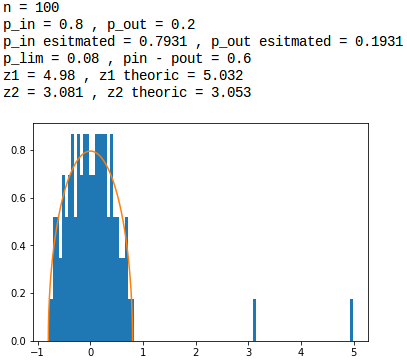
\includegraphics[scale=0.58]{static/spectral_n100_pin08_pout02.png}
		\caption{$n=100$, $\Delta p=0.6$}
		\label{n100delta05}
	\end{subfigure}
	\begin{subfigure}{.5\textwidth}
		\centering
		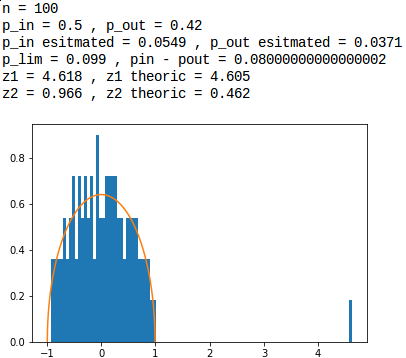
\includegraphics[scale=0.58]{static/spectral_n100_pin05_pout042.png}
		\caption{$n=100$, $\Delta p=0.08$}
		\label{n100delta008}
	\end{subfigure}
	\begin{subfigure}{.5\textwidth}
		\centering
		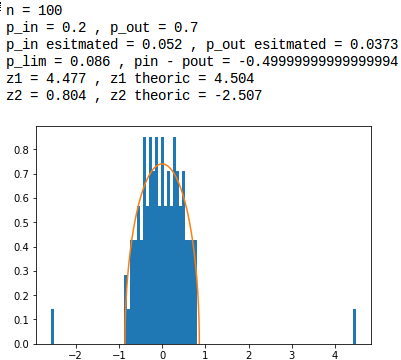
\includegraphics[scale=0.58]{static/spectral_n100_pin02_pout07.png}
		\caption{$n=100$, $\Delta p=-0.5$}
		\label{n100delta-05}
	\end{subfigure}
	\begin{subfigure}{.5\textwidth}
		\centering
		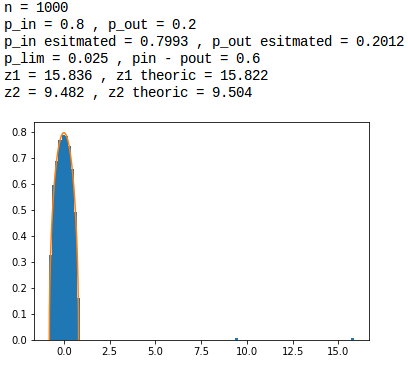
\includegraphics[scale=0.58]{static/spectral_n1000_pin08_pout02.png}
		\caption{$n=1000$, $\Delta p=0.6$}
		\label{n1000delta05}
	\end{subfigure}
	\begin{subfigure}{.5\textwidth}
		\centering
		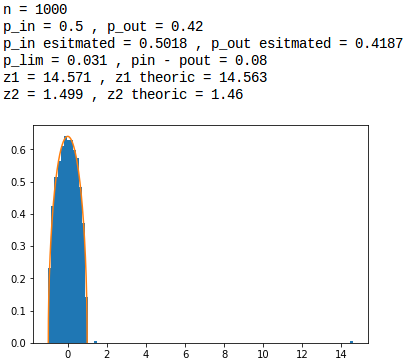
\includegraphics[scale=0.58]{static/spectral_n1000_pin05_pout042.png}
		\caption{$n=1000$, $\Delta p=0.08$}
		\label{n1000delta008}
	\end{subfigure}
	\begin{subfigure}{.5\textwidth}
		\centering
		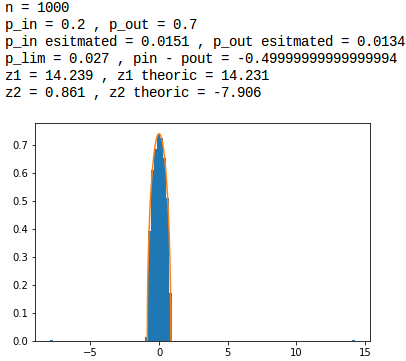
\includegraphics[scale=0.58]{static/spectral_n1000_pin02_pout07.png}
		\caption{$n=1000$, $\Delta p=-0.5$}
		\label{n1000delta-05}
	\end{subfigure}
\end{figure}
Le but est de générer une matrice d'adjacence A sous les mêmes hypothèses que \eqref{eq:1} en faisant varier les différents paramètres, à savoir: $n$, $p_{in}$, $p_{out}$ \\

\begin{figure}[H]
\centering
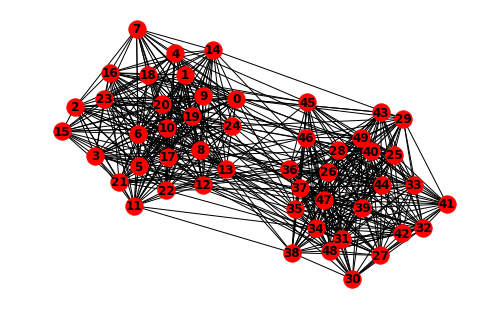
\includegraphics[scale=0.6]{static/graph_n50_pin08_pout01.png}
\caption{Graphe généré à partir des paramètres: $n=50$, $p_{in}=0.8$, $p_{out}=0.1$}
\end{figure}

\paragraph{ }\label{par: p_lim law}
L'élément discriminant du test spectral étant la variable $ \Delta p= p_{in} - p_{out}$, nous allons tester 3 valeurs représentatives des différents types de résultats:
\begin{itemize}
	\item[1-] $\Delta p \in [-1,\: -p_{lim}] \implies$ le graphe comporte de structure de communauté ``disassortative'';
	\item[2-] $\Delta p \in [-p_{lim},\: p_{lim}] \implies$ la méthode spectrale ne peut rien conclure sur la stucture de communauté du graphe;
	\item[2-] $\Delta p \in [p_{lim},\: 1] \implies$ le graphe comporte une structure de communauté ``assortative''.\\
\end{itemize}

Par la suite nous allons tester pour les valeurs $\Delta p= 0.5, 0.08, -0.5$ .
De plus nous ferons une première batterie de test avec $n=100$ et une autre avec $n=1000$.
La terminologie utilisée dans les figures ci-dessous est:
\begin{itemize} 
	\item[- \underline{$n,\: p_{in},\: p_{out},\: p_{lim},\: z_1,\: z_2$}:] sont identiques aux notations utilisées jusqu'à présent ;
	\item[- \underline{$z_1\: theoric, \:z_2\: theoric$}:] sont les plus grandes valeurs propres $z_1$ et $z_2$ calculées via les équations \eqref{z_1} et \eqref{z_2} ;    
	\item[- \underline{$p_{in}\: estimated, \:p_{out}\: estimated$}:] sont les probabilités du SBM calculées a posteriori grâce aux valeurs propres $z_1$ et $z_2$.\\
\end{itemize}
Les $p_{in}\: estimated, \:p_{out}\: estimated$ sont calculés via un calcul d'optimisation dont les conditions initiales sont $p_{in, 0} = 1$ et $p_{out, 0} = 0$.\\


La première observation que l'on peut faire est que les valeurs propres de nos matrices d'adjacence sont bien distribuées selon la loi du demi-cercle de Wigner.
De plus, en fonction de $\Delta p$ la mesure spectrale est perturbée (ou pas) par une ou deux valeurs propres qui sortent du support de la distribution initiale.\\

Dans les cas avec $\Delta p = 0.5$ (\autoref{n100delta05}, \autoref{n1000delta05}), on voit très clairement deux valeurs propres qui se détachent du support de la distribution de Wigner.
Les valeurs $z_1$, $z_2$ correspondent bien aux valeurs théoriques avec un taux d'erreur de l'ordre de $10^{-2}$.
Par conséquent lorsque l'on obtient une valeur propre négative, le modèle spectral nous permet de conclure qu'il y a une structure de communauté ``assortative'' dans le graphe.\\

Dans les cas avec $\Delta p = -0.5$ (\autoref{n100delta008}, \autoref{n1000delta008}), selon l'\autoref{z_2}, on ne s'attend à ce qu'une des valeurs propres théorique soit négative.
On observe une valeur propre négative en dehors du support de la loi de Wigner et une autre au dessus du support.
Ces valeurs observées correspondent on valeurs théoriques avec une erreur de l'ordre de $10^{-2}$.
Par conséquent lorsque l'on obtient une valeur propre négative, le modèle spectral nous permet de conclure qu'il y a une structure de communauté ``disassortative'' dans le graphe.\\

Enfin, les cas avec $\Delta p = 0.08$ (\autoref{n100delta-05}, \autoref{n1000delta-05}). 
On se trouve dans le cas limite décrit dans \autoref{subsec:1.3}, dans lequel le modèle ne peut pas interpréter les résultats du modèle spectral.
On peut observer sur la \autoref{n100delta-05} qu'il n'y a qu'une seule valeur propre qui est en dehors du support.
Par conséquent il n'y a qu'une seule valeur propre extrémale (ici $z_1$) qui correspond à sa valeur théorique, de fait nous ne pouvons conclure sur la structure de communauté du graphe.
Cependant, avec le même $\Delta p$ mais avec plus de nœud ($n = 1000$) le modèle spectral parvient à détecter la structure de communauté et à retrouver les valeurs $z_1$ et $z_2$.  
Ceci confirme la remarque du \autoref{rq:ngrand} selon laquelle, plus il y a d’information (i.e nœuds) dans le graphe plus la valeur de $p_{lim}$ tend vers $0$.\\

Si on compare les valeurs théoriques de l'article initial \cite{raj_rao} avec les valeurs des simulations, on voit très clairement une différence.\\
Par exemple, pour $p_{in} = 0.8$, $p_{out}=0.3$, et $n=100$ les valeurs propres calculées avec les équations \nameref{tab:bilan} sont $z_1 = 22.785$ et $z_2 = 18.815$.
Les valeurs propres empiriques sont $z_1 = 5.538$ et $z_2 = 2.545$.\\
Ou encore, pour $p_{in} = 0.2$, $p_{out}=0.7$, et $n=1000$ les valeurs propres calculées avec les équations \nameref{tab:bilan} sont $z_1 = -56.732$ et $z_2 = 31.833$.
Les valeurs propres empiriques sont $z_1 = 14.299$ et $z_2 = -7.934$.
\section{Erreurs de l'article}
Dans cette section, allons redémontrer les résultats obtenus dans le \autoref{tab:bilan} via la combinatoire.
Par la même occasion nous allons expliquer les erreurs commises dans l'article \cite[Graph spectra and the detectability of community structure in networks]{raj_rao}.
\subsection{Normalisation de la mesure spectrale de X}
Dans l'article l'équation $(7)$ donne la mesure spectrale de la matrice $X$.
\begin{align*}
	\rho(z) &= \frac{n}{\pi} \frac{\sqrt{2(c_{in} + c_{out}) - z^2}}{c_{in} + c_{out}}
\end{align*}
Calculons l'intégrale de $\rho(z)$. 
On sait que son support est $[a, b] = [-\sqrt{2(c_{in} + c_{out})},\sqrt{2(c_{in} + c_{out})}]$.
\begin{align*}
	\int_{a}^{b} \rho(z) \, \mathrm{d}z &= \int_{a}^{b} \frac{n}{\pi} \frac{\sqrt{2(c_{in} + c_{out}) - z^2}}{c_{in} + c_{out}}  \, \mathrm{d}z \\
	&= \int_{a}^{b} \frac{1}{\pi} \frac{\sqrt{2 n (p_{in} + p_{out}) - z^2}}{p_{in} + p_{out}}  \, \mathrm{d}z \\
	&= \int_{a}^{b} \frac{\sqrt{n}}{\pi} \frac{\sqrt{2 (p_{in} + p_{out}) - \frac{z^2}{n}}}{p_{in} + p_{out}}  \, \mathrm{d}z  \\
	&= n \int_{a'}^{b'} \frac{1}{\pi} \frac{\sqrt{2 (p_{in} + p_{out}) - u^2}}{p_{in} + p_{out}}  \, \mathrm{d}u  
\end{align*}
avec $u^2 = \frac{z^2}{n}$, $a'= \sqrt{2(p_{in} + p_{out})}$ et $b'= \sqrt{2(p_{in} + p_{out})}$.
Or la fonction sous l’intégrale correspond à la loi du demi-cercle de Wigner de paramètre $\sigma = (p_{in} + p_{out})$, qui est normalisée sur le fermé $[a', b']$.
On obtient donc:
\begin{align*}
 	\int_{a}^{b} \rho(z) \, \mathrm{d}z &= n
\end{align*}
Il y a donc un problème de normalisation.

\subsection{Choix de la variance des entrées de X}
Nous allons réécrire le raisonnement de l'article \cite[Graph spectra and the detectability of community structure in networks]{raj_rao} lorsque l'on souhaite déterminer la densité spectrale de $X$.\\

La transformé de Stieltjes de $X$ est :
\begin{equation}
	\rho(z) = \frac{1}{\pi} Im\langle Tr(zI - X)^{-1}\rangle
\end{equation}
où $\langle \dots \rangle$ indique la moyenne de l'ensemble.
On peut réécrire la trace de la moyenne comme ce qui suit: 
\begin{align}
	\langle Tr(zI - X)^{-1}\rangle &= \frac{1}{z}\sum_{k=0}^{\infty} \frac{Tr\langle X^k\rangle}{z^k} \\
	Tr\langle X^k\rangle &= \sum_{i_1\dots i_k}\langle X_{i_1i_2}X_{i_1i_2}\dots X_{i_ki_1}\rangle \label{eq: trace Xk}
\end{align}

D'après l'analyse préliminaire effectué \autoref{ch:Analyse spectrale de la matrice d'adjacence}, on sait que $X$ est centrée et que les $X_{ij} \; \forall i\leq j$ sont des variables de Bernoulli indépendantes définies celon \eqref{eq: X}.
Par conséquent $\langle X_{i_1i_2}X_{i_1i_2}\dots X_{i_ki_1}\rangle \neq 0$ si $k = 2m$ avec $m\in \mathbb{N}$ et si chaque $X_{ij}$ apparaît exactement deux fois.
De plus.
\begin{equation}
	\langle X_{ij}^2\rangle = \left\{
	\begin{array}{lr}
		\sigma_{in}^2  &\; si \; (i,j < \frac{n}{2}) \; ou \; (i,j \ge \frac{n}{2}) \\
		\sigma_{out}^2 &\; else \; where
	\end{array}
\right.\nonumber
\end{equation}

C'est à ce moment qu’apparaît l'erreur.  
En effet dans l'article ils choisissent comme variances des entrées de X: 
\begin{align*}
	\langle X_{ij}^2 \rangle = \frac{c_{in} + c_{out}}{2n} \;\; \forall \; i,j
\end{align*}
\subsection{Détermination de la mesure spectrale de X par la combinatoire}
Pour trouver la mesure spectrale de $X$, l'article utilise une méthode combinatoire.
Nous allons refaire le raisonnement en se basant sur la démonstration du théorème de Wigner par la combinatoire dans \cite[Introduction aux matrices aléatoires]{wigner}.\\
\section{Généralisation}
\subsection{Cas avec n communautés}
On peut a présent généraliser à un nombre de communautés $q \geq 2$.
Nous allons supposer que les communautés sont de même taille, à savoir $n_q = \frac{n}{q}$.
\paragraph{}\label{rq:contrainte model}
Une première contrainte apparaît, de par l'utilisation des théorèmes \ref{th:1} et \ref{th:2}, sur les valeurs des probabilités de la matrice d'adjacence $A$.
En effet, d'après le \autoref{th:1}, pour que la matrice $X$ est une mesure spectrale qui tende vers la loi de Wigner il faut que la norme 1 des vecteurs lignes de son profil de variance soient égales ($\parallel x \parallel_1 = \sum_{j=1}^{n}|x_j|$).
Par conséquent, si on veut augmenter le nombre de communautés $q$ dans le modèle, on est forcé de garder deux probabilités $p_{in}$ et $p_{out}$ qui jouent le même rôle que celles introduites précédemment (cf. \ref{rq:probability}).\\

On sait que la matrice d’adjacence du graphe sous le SBM à $q$ communautés est $A = X + \langle A \rangle$.  
Pour poursuivre l'analyse on va suivre la trame suivante:
\begin{itemize}
	\item[1-] Trouver l'équation de $\langle A \rangle$ ;
	\item[2-] Trouvez l'équation de X et déterminer son profil de variance ;
	\item[3-] Trouvez les $q$ valeurs propres associées aux perturbations de rang 1 ;
	\item[4-] Trouver $p_{lim}$.\\
\end{itemize}

% ------------------------------------------------- 1- trouver <A>  -------------------------------------------------
\subsubsection*{1- Équation de $\langle A \rangle$}
$\langle A \rangle$ étant symétrique, le théorème spectral nous dis qu'il existe une base orthonormée telle que $\langle A \rangle = \sum_{n}^{i=1}\lambda_i\mathbf{u}_i\mathbf{u}_i^{\star}$.
Après les calculs on trouve:
\begin{align} 
\langle A \rangle :&= n_q(p_{in} + (q-1)p_{out}) \mathbf{u}_1\mathbf{u}_1^{\star} + n_q(p_{in}-p_{out})\sum_{i=1}^{q-1}\mathbf{u}_i\mathbf{u}_i^{\star}\\
				   &= \frac{c_{in} + (q-1)c_{out}}{q} \mathbf{u}_1\mathbf{u}_1^{\star} + \frac{c_{in}-c_{out}}{q}\sum_{i=1}^{q-1}\mathbf{u}_i\mathbf{u}_i^{\star}
\end{align}\\
où les trois valeurs propres sont $0$, $n_q(p_{in} + (q-1)p_{out})$, $n_q(p_{in}-p_{out})$ de multiplicité $q(n_q - 1)$, $1$, $q-1$.\\

% ------------------------------------------------- 2- trouver X  -------------------------------------------------
\subsubsection*{2- Profil de variance de $\frac{X}{\sqrt{n}}$}
De la même manière que dans \autoref{ch:Analyse spectrale de la matrice d'adjacence} on trouve:
\begin{equation}
	X_{ij} \sim \left\{
	\begin{array}{lr}
		\sigma_{in} Z_{ij} & : (i,j \in P_{in}) \\
		\sigma_{out} Z_{ij} & : (i,j \in P_{out})
	\end{array}
\right.\nonumber
\end{equation}
Où $Z_{ij} = \frac{B_{ij}(p) - p}{\sqrt{p(1-p)}} \;\;avec \; p = p_{in} \; ou \; p_{out}$, $B_{ij}(p) \sim B(p)$, $B(p)$ loi de Bernoulli de paramètre p\\
La somme de n'importe quel vecteur ligne (ou colonne) du profil de variance de $\frac{X}{\sqrt{n}}$ est égale à : 
\begin{align}
\label{eq:sigma2} 
\sigma^2 = \frac{\sigma_{in}^2 + (q-1)\sigma_{out}^2}{q}
\end{align}
Le profil de variance de $\frac{X}{\sqrt{n}}$ est donc une matrice bi-stochastique.\\
% ------------------------------------------------- 3- trouver les vp -------------------------------------------------
\subsubsection*{3- Valeurs propres de $\frac{A}{\sqrt{n}}$}
Soit $\lambda$ une valeur propre de $\frac{A}{\sqrt{n}}$ et le vecteur propre associé.
\begin{align}
&\Leftrightarrow \frac{A}{\sqrt{n}}v =\lambda v \nonumber \\
&\Leftrightarrow (\Gamma - \lambda I)v =-\alpha \mathbf{11}^Tv - \beta \sum_{i=1}^{q-1}\mathbf{u}_i\mathbf{u'}_i^T \label{eq:generalize}
\end{align}
Pour trouver la valeur propre associée à $\mathbf{u}_1$ on multiplie à gauche par $\mathbf{u}_1^{\star}(\Gamma -\lambda I)^{-1}$ et on obtient:
\begin{align}
\eqref{eq:generalize} &\Leftrightarrow \mathbf{u}_1^{\star}v =-\alpha \mathbf{u}_1^{\star}(\Gamma -\lambda I)^{-1}\mathbf{u}_1\mathbf{u}_1^{\star}v - \beta \mathbf{u}_1^{\star}(\Gamma -\lambda I)^{-1}\sum_{i=1}^{q-1}\mathbf{u}_i\mathbf{u}_i^{\star}v \nonumber\\
&\xrightarrow[n \to +\infty]{} 1 = -\alpha g_{wig}^{\sigma^2}(\lambda) \nonumber\\
&\Leftrightarrow 1 = \alpha \frac{\lambda + \sqrt{\lambda^2 - 4\sigma^2}}{2\sigma^2} \nonumber\\
&\Leftrightarrow \lambda = \frac{c_{in} + (q-1)c_{out}}{q\sqrt{n}} + \frac{q\sqrt{n}\sigma^2}{c_{in} + (q-1)c_{out}} \label{eq:z_2 generalize}
\end{align}
Si on remplace $q$ par $2$ on retrouve l'équation \eqref{z_2}.\\
Pour trouver les valeurs propres associée aux $\mathbf{u}_i, \; \forall i \in \{2, \cdots, q-1\}$ on multiplie à gauche par $\mathbf{u}_2^{\star}(\Gamma -\lambda I)^{-1}$ et on obtient:
\begin{align}
\eqref{eq:generalize} &\Leftrightarrow \mathbf{u}_2^{\star}v =-\alpha \mathbf{u}_2^{\star}(\Gamma -\lambda I)^{-1}\mathbf{u}_1\mathbf{u}_1^{\star}v - \beta \mathbf{u}_2^{\star}(\Gamma -\lambda I)^{-1}\sum_{i=1}^{q-1}\mathbf{u}_i\mathbf{u}_i^{\star}v \nonumber\\
&\xrightarrow[n \to +\infty]{} 1 = -\beta g_{wig}^{\sigma^2}(\lambda) \nonumber\\
&\Leftrightarrow 1 = \beta \frac{\lambda + \sqrt{\lambda^2 - 4\sigma^2}}{2\sigma^2} \nonumber\\
&\Leftrightarrow \lambda = \frac{c_{in} - c_{out}}{q\sqrt{n}} + \frac{q\sqrt{n}\sigma^2}{c_{in} - c_{out}}\label{eq:z_1 generalize}
\end{align}
Si on remplace $q$ par $2$ on retrouve l'équation \eqref{z_1}.\\
Les valeurs propres de $A$ pour les valeurs propres de $\langle A \rangle$ égales à zéros appartiennent au support de la distribution de Wigner.
Elles n'apportent donc aucune information supplémentaire sur la structure de communauté du graphe étudié.\\   

Nous noterons $z_1 =$ \eqref{eq:z_1 generalize}  et $z_2 =$ \eqref{eq:z_2 generalize} pour la suite.
 

% ------------------------------------------------- 4- trouver p_lim -------------------------------------------------
\subsubsection*{4- Seuil de décidabilité $p_{lim}$}
Nous cherchons maintenant à déterminer $p_{lim}$.
La condition limite naturelle est celle où la valeur propre $z_2$ qui sort du support de la distribution de Wigner est égale au bord droit du support de la mesure spectrale de la matrice A.
On a alors 
\begin{align*}
	&\Leftrightarrow \lambda^+ = z_1\\
	&\Leftrightarrow 2 \sigma = \frac{c_{in} - c_{out}}{q\sqrt{n}} + \frac{q\sqrt{n}\sigma^2}{c_{in} - c_{out}}\\
	&\Leftrightarrow 0 = \beta \sigma^2 - 2 \sigma + \alpha \\
	&\Leftrightarrow p_{in} - p_{out} = \frac{q\sigma}{\sqrt{n}}  \\
\end{align*}
Donc
\begin{equation}
	p_{lim} = \frac{\sqrt{q(\sigma_{in}^2 + (q-1)\sigma_{out}^2)}}{\sqrt{n}} = \frac{q\sigma}{\sqrt{n}}  \\
\end{equation}


% ------------------------------------------------- 5- résumer -------------------------------------------------
\subsection{Bilan}
Ci-dessous le bilan de la généralisation:
\begin{align*}
	\sigma^2&: \frac{\sigma_{in}^2 + (q-1)\sigma_{out}^2}{q} \\
	z_1&: \frac{c_{in} - c_{out}}{q\sqrt{n}} + \frac{q\sqrt{n}\sigma^2}{c_{in} - c_{out}}\\
	z_2&: \frac{c_{in} + (q-1)c_{out}}{q\sqrt{n}} + \frac{q\sqrt{n}\sigma^2}{c_{in} + (q-1)c_{out}}\\
	p_{lim}&: \frac{\sqrt{q(\sigma_{in}^2 + (q-1)\sigma_{out}^2)}}{\sqrt{n}} \\
\end{align*}

% ------------------------------------------------- 6- Simulation -------------------------------------------------
\subsection{Simulations}
\begin{figure}[H]
\centering
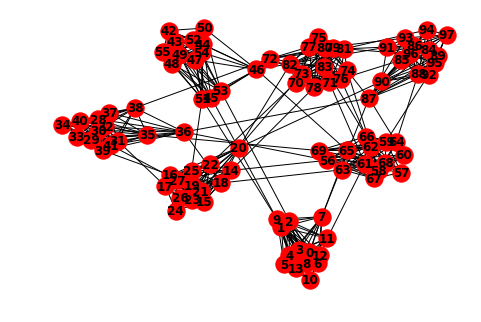
\includegraphics[scale=0.6]{static/graph_q7_n100_pin08_pout0011.png}
\caption{Graphe généré à partir des paramètres: $q=7$ $n=100$, $p_{in}=0.8$, $p_{out}=0.01$}
\end{figure}
\begin{figure}[H]
\centering
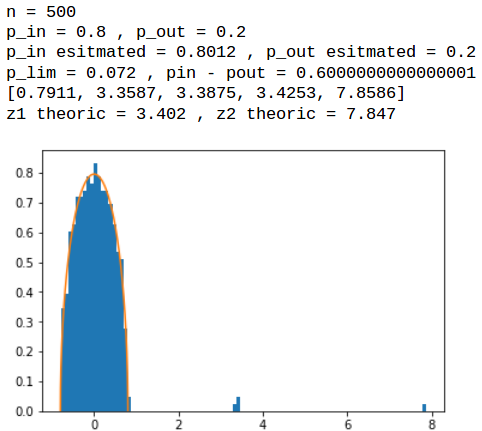
\includegraphics[scale=0.6]{static/spectral_q4_n500_pin08_pout02}
\caption{$q=4$, $n=500$, $\Delta p=0.6$}
\label{n500delta-05}
\end{figure}
\subsection{Limites du modèle}
Le première limite de ce modèle est que l'on est cantonné à des communautés de même taille $n_q$.
En effet si on change ce paramètre pour chacune des communautés alors le \autoref{th:1} n'est plus applicable, la somme des éléments de chaque vecteurs ligne du profil de variance n'est plus constant.\\

La deuxième contrainte est le fait que l'on doit toujours garder deux paramètres $p_{in}$ et $p_{out}$ indépendamment du nombre de communautés $n_q$ et du nombre de nœuds dans le graphe $n$.
Idéalement nous souhaiterions avoir un paramètre $p_{ij}$ correspondant à la probabilité d'avoir une arrête entre le nœud $i$ et le nœud $j$ et ce $\forall i<j$.\\
Une manière d'encoder ces paramètres est d'utiliser la relation suivante $p_{ij} = q_iq_jC_{\alpha}$
\begin{align}
	p_{ij} &= q_iq_jC_{g_ig_j}
\end{align}
Où $q_i$ est la probabilité intrinsèque du nœud $i$ à avoir une arrête, $g_i$ est la communauté correspondant au nœud $i$ et $C_{g_ig_j}$ est le facteur de correction par communauté.\\
Cette formalisation plus générale est très répandu dans la théorie de la détection de communauté spectrale.
\nocite{*}

\part{Analyse d'algorithmes de graph spectral clusturing}
\section{Bethe Hessian}
\subsection{Principe}
Dans le contexte d'un SBM à 2 communautés 
\subsection{Simulations}
\begin{figure}[H]
	\begin{subfigure}{.5\textwidth}
		\centering
		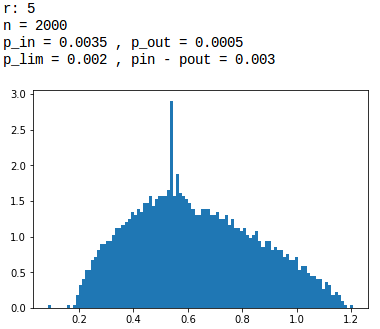
\includegraphics[scale=0.58]{static/bh_5.png}
		\label{bh5}
	\end{subfigure}
	\begin{subfigure}{.5\textwidth}
		\centering
		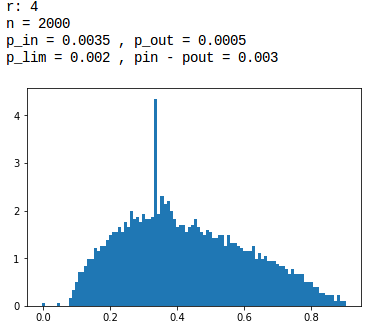
\includegraphics[scale=0.58]{static/bh_3.png}
		\label{bh3}
	\end{subfigure}
	\begin{subfigure}{.5\textwidth}
		\centering
		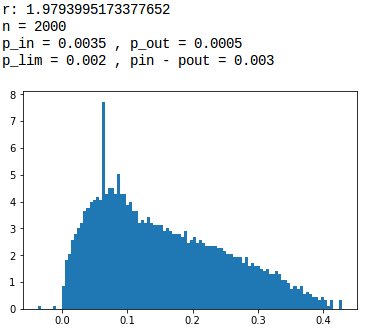
\includegraphics[scale=0.58]{static/bh_2.png}
		\label{bh2}
	\end{subfigure}
	\begin{subfigure}{.5\textwidth}
		\centering
		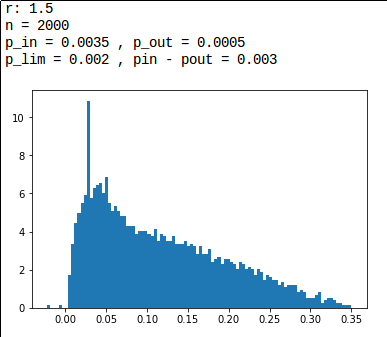
\includegraphics[scale=0.58]{static/bh_1_5.png}
		\label{bh15}
	\end{subfigure}
	\begin{subfigure}{.5\textwidth}
		\centering
		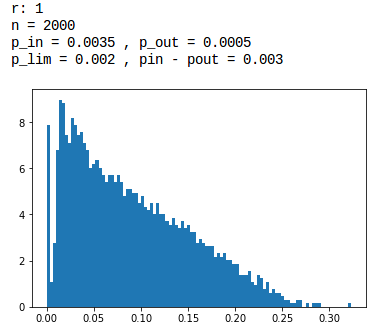
\includegraphics[scale=0.58]{static/bh_1.png}
		\label{bh1}
	\end{subfigure}
	\begin{subfigure}{.5\textwidth}
		\centering
		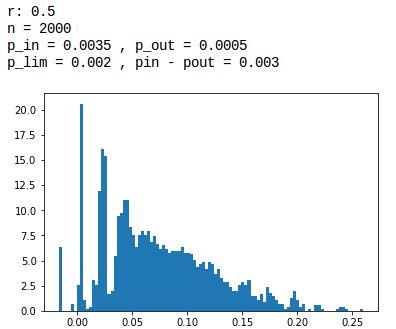
\includegraphics[scale=0.58]{static/bh_0_5.png}
		\label{bh05}
	\end{subfigure}
\end{figure}
\subsection{Theorie}
\section{Modularity Matrix}


\appendix
\section{Valeurs propres obtenues via algèbre linéaire}\label{annexe: A}
Dans cette annexe nous allons trouver les valeurs propres de l'\autoref{eq: A generalize}.

On a 
\begin{align*}
	\langle A \rangle = \theta_q \otimes \mathbf{1}_{n_q} \mathbf{1}_{n_q}^t
\end{align*}
avec $\theta_q$ une matrice $q \times q$, dont les éléments diagonaux sont égaux à $a$ et les autres sont égaux à $b$, $\mathbf{1}_{n_q}$ le vecteur colonne rempli de $1$ et de taille $n_q$, et $\otimes$ est le produit de Kronecker.\\
On cherche les valeurs propres de $\langle A \rangle$: 
\begin{align*}
	&\Leftrightarrow 
		|\A - \lambda I_n| = 0\\
	&\Leftrightarrow 
		det(\theta_q \otimes \mathbf{1}_{n_q} \mathbf{1}_{n_q}^t - \lambda I_n) = 0
\end{align*}
On a 
\begin{align*}
	det(\A) &= 
\begin{vmatrix}
B & C &  \dots & \dots & C \\ 
C & \ddots &  & & \vdots \\ 
\vdots &  &  & \ddots & C \\ 
C & \ldots & \ldots & C & B
\end{vmatrix} \\
\end{align*}
Où $B = a\mathbf{1}_{n_q} \mathbf{1}_{n_q}^t - \lambda I_{n_q}$ et $C = b \mathbf{1}_{n_q} \mathbf{1}_{n_q}^t$.\\

On a la formule de déterminant par blocs suivante: 
\begin{align*}
det \left(\begin{matrix} A & 0 \\ C & D \end{matrix} \right) = det(A)det(D)
\end{align*}
et en utilisant les combinaisons linaires lignes/colonnes suivantes $q-2$ fois
\begin{align}\label{eq: matrix method}
	(L_n \leftarrow L_n  - L_{n-1}) \\
	(C_{n-1} \leftarrow C_{n-1}  + C_n) \nonumber
\end{align}
on obtient
\begin{align*}
	det(\A ) &= 
	\begin{vmatrix}
	B & (q-1)C\\
	C & B + (q-2)C
	\end{vmatrix}
	| B - C |^{q-2} \\
	 &= F_{n_q}G_{n_q}^{q-2}
\end{align*}

Commençons par factoriser le polynôme $G_{n_q}^{q-2}$.
En utilisant la même stratégie que \eqref{eq: matrix method}, on obtient:
\begin{align*}
	G_{n_q} = (-\lambda)^{n_q - 1} (\lambda - n_q(a-b))
\end{align*}

Même stratégie pour $F_{n_q}$ et $H_{n_q}$ qui suit, on obtient: 
\begin{align*}
	F_{n_q} &= (-\lambda)^{n_q - 1} H_{n_{q}}\\
	H_{n_{q}} &= 
	\begin{vmatrix}
	A & n_{q}(q-1)\mathbf{1}_{n_q} \\
	b\mathbf{1}_{n_q}^t  &  n_q(a + (q-2)b) - \lambda
	\end{vmatrix}\\
	&= (-\lambda)^{n_q - 1}E_{n_q}\\
	&= (-\lambda)^{n_q - 1}(\lambda - n_q(a + (q-1)b))(\lambda - n_q(a-b)) 
\end{align*}
On a donc au final
\begin{equation}
	\boxed{det(\A - \lambda I_n) = (-\lambda)^{q(n_q -1)}(\lambda - n_q(a-b))^{q-1}(\lambda - n_q(a + (q-1)b)) }
\end{equation}
Donc les trois valeurs propres de la matrice $\A$ sont $0$, $n_q(p_{in} + (q-1)p_{out})$, $n_q(p_{in}-p_{out})$ de multiplicités respectives $q(n_q - 1)$, $1$, $q-1$.\\
\part{Conclusion}
\section*{Bilan}
Nous avons réussi à redémontrer les résultats de l'article \cite{raj_rao}.
L'intérêt de ces nouveaux résultats réside dans la nouvelle limite de cet algorithme de détection de communauté que nous avons trouvé.
En effet, cette limite est largement citée et réutilisée dans les articles de ``graphe spectral clustering''.

Une perspective serait de réétudier les quelques articles qui utilisent comme base l’ancienne limite et ainsi corriger les résultats dont ils dérivent.\\

Nous avons aussi étudié d'autres algorithmes spectraux plus fins doté d'un performance supérieur.
Les recherches récentes dans ce domaine se tournent principalement sur la ``Non-Backtracking Matrix''.
Ceci est dû à ces propriétés plus intéressantes que celle des autres opérateurs linéaires (e.g matrice d'adjacence).
Mais aussi et surtout grâce au fait qu'elle à des connections avec des théories en physique comme les modelés d'Ising.

\section*{Remerciement}
Je tiens à remercier Jamal Najim pour m'avoir aiguillé et soutenu tout au long de ce stage.
Ses conseils ont été essentiels à l'aboutissement de ce mémoire.

\newpage

\bibliographystyle{plain}
\bibliography{b}
\end{document}
